\documentclass{article}

\usepackage{amsmath}

\usepackage{mathptmx}           
\usepackage{graphicx}           
\usepackage{url}            
\usepackage{subcaption}    

\usepackage[a4paper,margin=2cm]{geometry}

\usepackage{natbib} 
\usepackage[numbered, framed]{mcode}

\usepackage{lipsum}

\begin{document}

\author{H. Blum, D. Cavezza, A. Paudice and M. Rohbeck\\
 Machine Learning CO395\\
  Imperial College London}
\date{\today}
\title{Assignment 2: Decision Trees Algorithm}
\maketitle

\section{Training}
Decision trees are a conceptually simple, yet powerful model for solving classification problems. The ID3 algorithm is one of the simplest training algorithms for decision trees: it builds the tree by choosing at each step the attribute that maximizes the Information Gain, a measure that represents the discriminatory power of an attribute over the class values.\\
The problem we are given consists in classifying facial expressions into 6 emotion classes via decision trees; each facial expression is represented as a feature vector of 45 Action Units (AU), where each feature is a binary value that indicates the presence or absence of each AU in the example. We decompose the problem in 6 binary decision problems, one corresponding to the recognition of one specific emotion. Therefore, we use ID3 to train 6 different trees, each specific to one emotion.\\
Our implementation of ID3 is provided in the files \verb$train.m$, \verb$DTTrain.m$, \verb$choose_best_attr.m$, and \verb$sample_entropy.m$, containing the functions with the same name.\\
The function \verb$train$ is the entry point for the training algorithm. It takes as inputs the training examples, the array of attribute ids (in our case, an array from 1 to 45), and an array of labels of the same length as the number of examples; such labels are numbers from 1 to 6, each one indicating one of the emotions in the original dataset. It returns the 6 desired trees.\\
Each tree is trained on a transformed version of the input data: at the i-th iteration of the for loop, the labels are made binary; the vector \verb$binary_targets$ contains a 1 in the positions corresponding to the i-th emotion, a 0 in all the other positions. The function \verb$DTTrain$ is called to train each tree on such transformed data.
\begin{lstlisting}
function [ T ] = train( examples, attributes, labels )
%Train 6 binary trees on the training set (examples, labels) and return
%them into the tree array T.

[m, n] = size(examples); 
binary_targets = zeros(m, 1);

for i = 1:6
   
    %Switch to binary labels
    index = find(labels == i);
    binary_targets(index) = 1;
    
    %Train a tree to learn an emotion
    T(i) = DTTrain(examples, attributes, binary_targets);
    
%    DrawDecisionTree(T(i));
    
    binary_targets = zeros(m, 1);
    
end

end
\end{lstlisting}
The function \verb$DTTrain$ is a recursive function implementing the ID3 algorithm. Every time a recursion occurs, a check is performed on the entropy of the current node: if it is not 0, the attribute that maximizes the Information Gain is chosen and associated to the current node, then the recursion occurs.\\
In the first call it is passed the whole training sample, the array 1:45 of attribute ids, and the binary labels.
\begin{lstlisting}
function [ tree ] = DTTrain( examples, attributes, binary_targets )
%Train a decision tree on the dataset (examples, binary_target)
%according to the ID3 algorithm. The examples have the attributes listed in
%attributes
\end{lstlisting}
First, an empty tree is initialized.
\begin{lstlisting}[firstnumber=6]
%Initialize an empty tree
tree.op = [];

tree.kids = [];
tree.class = [];
\end{lstlisting}
Then a check on the input's entropy is performed. If the sample entropy in the labels is 0, the algorithm is in a pure node, that is all the current examples belong to the same class: in such case, the algorithm must stop, and the value returned by the current node is the class value held by the majority of the examples. Likewise, the algorithm must stop if there are no more attributes to decide about. In these cases, \verb$tree.op$ and \verb$tree.kids$ are not set, so as to mark the node as a leaf.
\begin{lstlisting}[firstnumber=12]
if (sample_entropy(binary_targets) == 0 || isempty(attributes))   
    % either pure targets or no more attributes to base decision on
    
    tree.class = maj_value(binary_targets);
\end{lstlisting}
Else, the attribute that yields the highest Information Gain is chosen
\begin{lstlisting}[firstnumber=17]
else
    
    tree.op = choose_best_attr(examples, attributes, binary_targets);
\end{lstlisting}
and the examples are split by the value they contain in the chosen attribute.
\begin{lstlisting}
    tree.kids = cell(1, 2);
        
    % raise up the kids
    
    for j = 1:2
        
        %fprintf('#Examples: %d \n', length(examples));
        child_index = find(examples(:, tree.op) == (j - 1));
        child_examples = examples(child_index, :);     
        child_binary_targets = binary_targets(child_index);
\end{lstlisting}
At this point, the set of examples with a specific value of the chosen attribute may be empty. In that case, the corresponding kid node is made leaf and the returned class value is the value held by the majority of the nodes in the current node.
\begin{lstlisting}[firstnumber=36]
        if (isempty(child_examples))
            % we can't train this child, make a leaf with the majority
            % value of all training data coming to the parent
            
            tree.kids{j}.op = [];
            tree.kids{j}.kids = [];
            tree.kids{j}.class = maj_value(binary_targets);
\end{lstlisting}
Otherwise, the corresponding subtree is created. Note that in the recursive calls, the chosen attribute is deleted from the list of candidate attributes, since its value is fixed for the samples in each of the kids (0 for the left kid and 1 for the right).
\begin{lstlisting}[firstnumber=44]
        else 
            
            % remove the used attribute from the list
            index = find(attributes == tree.op);
            attributes(index) = [];
            
            % recursive training with this child
            tree.kids{j} = DTTrain(child_examples, attributes, ...
                child_binary_targets);
                    
        end
\end{lstlisting}
At line 19, the above functions calls \verb$choose_best_attr$. This function computes the Information Gain of every available attribute and returns the id of the attribute that yields the highest Information Gain.
\begin{lstlisting}
function [ best_attr ] = choose_best_attr( examples, attributes, binary_targets )
%chooseBestAtt computes and return in bestAtt the attribute in attributes
%which determine the maximum information gain for the set 
%(examples, binary_targets). Return -1 if the set is pure because no split
%is required

%Compute the sample entropy
n_ex = length(binary_targets);         %Dataset size
E = sample_entropy(binary_targets); %Sample entropy

% initial values
best_gain = 0;
best_attr = attributes(1); % for now this is as good as anything
    
for i = 1:length(attributes)
       
    % examples where attribute is 1
    one_attr = binary_targets(examples(:, attributes(i)) == 1); 
    % examples where attribute is 0
    zero_attr = binary_targets(examples(:, attributes(i)) == 0);
        
    E_partition = length(one_attr)/n_ex * sample_entropy(one_attr) ...
        + length(zero_attr)/n_ex * sample_entropy(zero_attr);
        
    gain = E - E_partition;
        
    if (gain > best_gain)
            
       best_gain = gain;
       best_attr = attributes(i);
        
    end
        
end

end

\end{lstlisting}
Finally, the files \verb$sample_entropy.m$ and \verb$maj_value.m$ simply contain the computation of the entropy and the most frequent label value in a sample respectively.

\section{Decision making strategies}
Since we have different trees, and each of these trees may commit mistakes in its classification, their outputs may be contradictory. Specifically, more than one tree may return 1 in response to the same example, or all trees may return 0. Therefore, we have devised different decision policies to resolve conflicts.

\subsection{Random choice}
One possible strategy is choosing randomly: if more than a tree returns 1, the label of the example is chosen randomly among the classes corresponding to such trees; if all the trees return 0, the label is picked randomly among all the classes.\\
The implementation of this strategy is in the file \verb$testTreesRandomChoice.m$.
\begin{lstlisting}
function [ predictions ] = testTreesRandomChoice(T,x2)
% TestTreesRandomChoice performs a random selection among the emotions of
% all the trees that return a prediction of 1, or among all the emotions if
% all the trees return 0.

[m,n] = size(x2);
binary_predictions = zeros(m,6);
predictions = zeros(m,1);

for i = 1:m
    for j = 1:6
        binary_predictions(i,j) = predictionBinaryTree(T(j),x2(i,:));
    end
    % If all the predictions are 0, pick an emotion randomly
    if(max(binary_predictions(i,:))==0)
        predictions(i) = randi(6);
    % Else pick an emotion randomly among the 1s
    else
        candidateEmotions = find(binary_predictions(i,:));
        predictions(i) = candidateEmotions(randi(length(candidateEmotions)));
    end
    
end


end
\end{lstlisting}
The function \verb$predictionBinaryTree$ called in line 12 is defined in the same file: it passes through the branches of the tree corresponding to the attribute values of the input example and returns the binary label corresponding to the reached leaf.
\begin{lstlisting}[firstnumber=28]
function [ class ] = predictionBinaryTree( tree, x )
%predictionBinaryTree walks along the tree to find the classification of
%the istance x
    
    if (isempty(tree.op))   %Check if it is a leaf
        
        class = tree.class;
        
    else                    %Test the attribute
        
        x_to_test = x(tree.op);
        
        if (x_to_test == 0) %Follow the left branch
           
           class = predictionBinaryTree(tree.kids{1}, x);
            
        else %Follow the right branch
            
           class = predictionBinaryTree(tree.kids{2}, x);
            
        end
        
    end

end
\end{lstlisting}
This strategy is one of the simplest to consider in resolving conflicts. It is chosen as our baseline strategy.

\subsection{Score-based choice}

\subsection{Tree confidence strategy}

\section{Cross-validation}


\section{Performance}


\section{Questions}





=================================================
\section{Implementations}
From the set of 6 Decision Trees, each tree will return a binary classification for a given data sample. Therefore, we need an Algorithm that decides on Basis of the output of the 6 trees, which class the given sample falls into. In fact, this algorithm does not even have to depend on the output of the classification trees. For example, one could think of an algorithm that simply outputs a randomly choosen classification and will have an accuracy of 17\% for a balanced test set. However, we searched for algorithms with a better performance.


\subsection{Stacking}
As we already implemented the basis function to train a decision tree, we tried to approximate the decision function (the function which outputs a class for a given example) by another tree which is trained on basis of the output of all 6 binary classification trees for the training set.
Therefore, given a sample, the decision algorithm works as follows:
\begin{enumerate}
    \item give the sample to the 6 binary classification trees
    \item give the output of all 6 trees to the decision function tree and output it's output
\end{enumerate} 

\subsubsection{Statistics}
The stacked tree method achieves a general accuracy of 72.4\% on clean data and 58.8\% in noisy data.

\begin{figure}[h]
    \hspace*{\fill}%
    \subcaptionbox{confusion matrix for clean data}{
        $\begin{bmatrix} 105 & 9 & 2 & 1 & 9 & 6\\ 37 & 145 & 1 & 5 & 3 & 7\\ 21 & 4 & 79 & 1 & 4 & 10\\ 13 & 10 & 4 & 177 & 5 & 7\\ 39 & 13 & 3 & 6 & 64 & 7\\ 18 & 5 & 13 & 6 & 8 & 157 \end{bmatrix}$
    }\hfill%
    \subcaptionbox{performance for the different classes with clean data}{
        \begin{tabular}{c | c c c}
        Class & Precision & Recall & $F_1$ \\
        \hline \hline
        1 & 48.3\% & 79.6\% & 57.6\% \\ 
        2 & 78.5\% & 73.7\% & 75.5\% \\ 
        3 & 76.5\% & 64.9\% & 69.8\% \\ 
        4 & 90.4\% & 82.5\% & 86.0\% \\ 
        5 & 66.3\% & 47.6\% & 54.7\% \\ 
        6 & 85.8\% & 76.4\% & 79.7\% \\ 
        \end{tabular}
    }%
    \hspace*{\fill}
    \\
    \hspace*{\fill}%
    \subcaptionbox{confusion matrix for noisy data}{
        $\begin{bmatrix} 19 & 7 & 16 & 4 & 9 & 33\\ 13 & 130 & 7 & 8 & 2 & 27\\ 13 & 16 & 98 & 11 & 4 & 45\\ 10 & 14 & 13 & 141 & 1 & 30\\ 21 & 8 & 4 & 6 & 43 & 28\\ 13 & 8 & 21 & 9 & 11 & 158  \end{bmatrix}$
    }\hfill%
    \subcaptionbox{performance for the different classes with noisy data}{
        \begin{tabular}{c | c c c}
        Class & Precision & Recall & $F_1$ \\
        \hline \hline
        1 & 23.5\% & 21.6\% & NaN\% \\ 
        2 & 70.2\% & 68.1\% & 68.8\% \\ 
        3 & 60.8\% & 51.1\% & 54.8\% \\ 
        4 & 78.1\% & 67.6\% & 72.0\% \\ 
        5 & 59.9\% & 38.1\% & 45.4\% \\ 
        6 & 49.1\% & 71.8\% & 57.7\% \\ 
        \end{tabular}
    }%
    \hspace*{\fill}
    
    \caption{statistics of the stacked tree}
\end{figure}





\subsection{Probabilistic Trees}
In this implementation, we assign a score to each leaf of every tree between 0 and 1. The score is correlated to the number of training examples that can be classified by the given leaf with respect to the total number of training examples in every class.
\begin{align*}
    \textrm{score} = \frac{\textrm{\# correctly classified training data by this leaf}}{\textrm{\# training data in this tree}}
\end{align*}
Of all binary classification trees returning 1, the decision algorithm will pick the class corresponding to the tree with the highest decision score. If no tree returns 1, it will pick at random.
\begin{lstlisting}
function [ predictions ] = decide_by_score(trees, testset)
% decide_by_score performs a classification based on the fraction of
% correctly classified training examples given by the tree leafs

[m,n] = size(testset);
predictions = zeros(m,1);

for i = 1:m
    % test in all trees, find the one with the best score
    best_score = 0;
    predictions(i) = NaN;
    for t = 1:6
        [pred, score] = prediction_with_score(trees(t),testset(i,:));
        if pred == 1
            % the tree recognises this item as his class
            if score > best_score
                predictions(i) = t;
                best_score = score;
            end
        end
    end
    % If all the predictions are 0, pick a random class
    if(isnan(predictions(i)))
        predictions(i) = randi(6);
    end
end

end
\end{lstlisting}


\subsubsection{Statistics}
The described method achieves a general accuracy of 73.2\% on clean data and 64.4\% in noisy data.

\begin{figure}[h]
    \hspace*{\fill}%
    \subcaptionbox{confusion matrix for clean data}{
        $\begin{bmatrix} 88 & 15 & 7 & 4 & 11 & 7\\ 15 & 145 & 5 & 7 & 14 & 12\\ 7 & 5 & 83 & 2 & 5 & 17\\ 4 & 8 & 6 & 188 & 5 & 5\\ 15 & 19 & 2 & 10 & 73 & 13\\ 3 & 9 & 14 & 11 & 4 & 166 \end{bmatrix}$
    }\hfill%
    \subcaptionbox{performance for the different classes with clean data}{
        \begin{tabular}{c | c c c}
        Class & Precision & Recall & $F_1$ \\
        \hline \hline
        1 & 66.3\% & 63.1\% & 63.4\% \\ 
        2 & 72.4\% & 75.1\% & 73.3\% \\ 
        3 & 67.1\% & 65.9\% & 66.2\% \\ 
        4 & 79.1\% & 84.0\% & 81.0\% \\ 
        5 & 60.5\% & 55.1\% & 57.5\% \\ 
        6 & 83.3\% & 81.1\% & 82.0\% \\
        \end{tabular}
    }%
    \hspace*{\fill}
    \\
    \hspace*{\fill}%
    \subcaptionbox{confusion matrix for noisy data}{
        $\begin{bmatrix} 21 & 11 & 20 & 8 & 19 & 9\\ 16 & 132 & 13 & 15 & 6 & 5\\ 14 & 13 & 108 & 22 & 11 & 19\\ 8 & 13 & 10 & 161 & 10 & 7\\ 15 & 10 & 8 & 7 & 59 & 11\\ 13 & 9 & 14 & 10 & 10 & 164 \end{bmatrix}$
    }\hfill%
    \subcaptionbox{performance for the different classes with noisy data}{
        \begin{tabular}{c | c c c}
        Class & Precision & Recall & $F_1$ \\
        \hline \hline
        1 & 25.5\% & 23.3\% & NaN \\ 
        2 & 71.4\% & 69.7\% & 69.9\% \\ 
        3 & 64.4\% & 56.7\% & 59.2\% \\ 
        4 & 71.6\% & 77.6\% & 74.0\% \\ 
        5 & 51.0\% & 52.9\% & 50.7\% \\ 
        6 & 76.2\% & 74.1\% & 74.6\% \\
        \end{tabular}
    }%
    \hspace*{\fill}
    
    \caption{statistics on the probabilistic tree}
\end{figure}


\section{Pruning}
\begin{figure}
\centering
\subcaptionbox{Pruning Example with clean data}{
    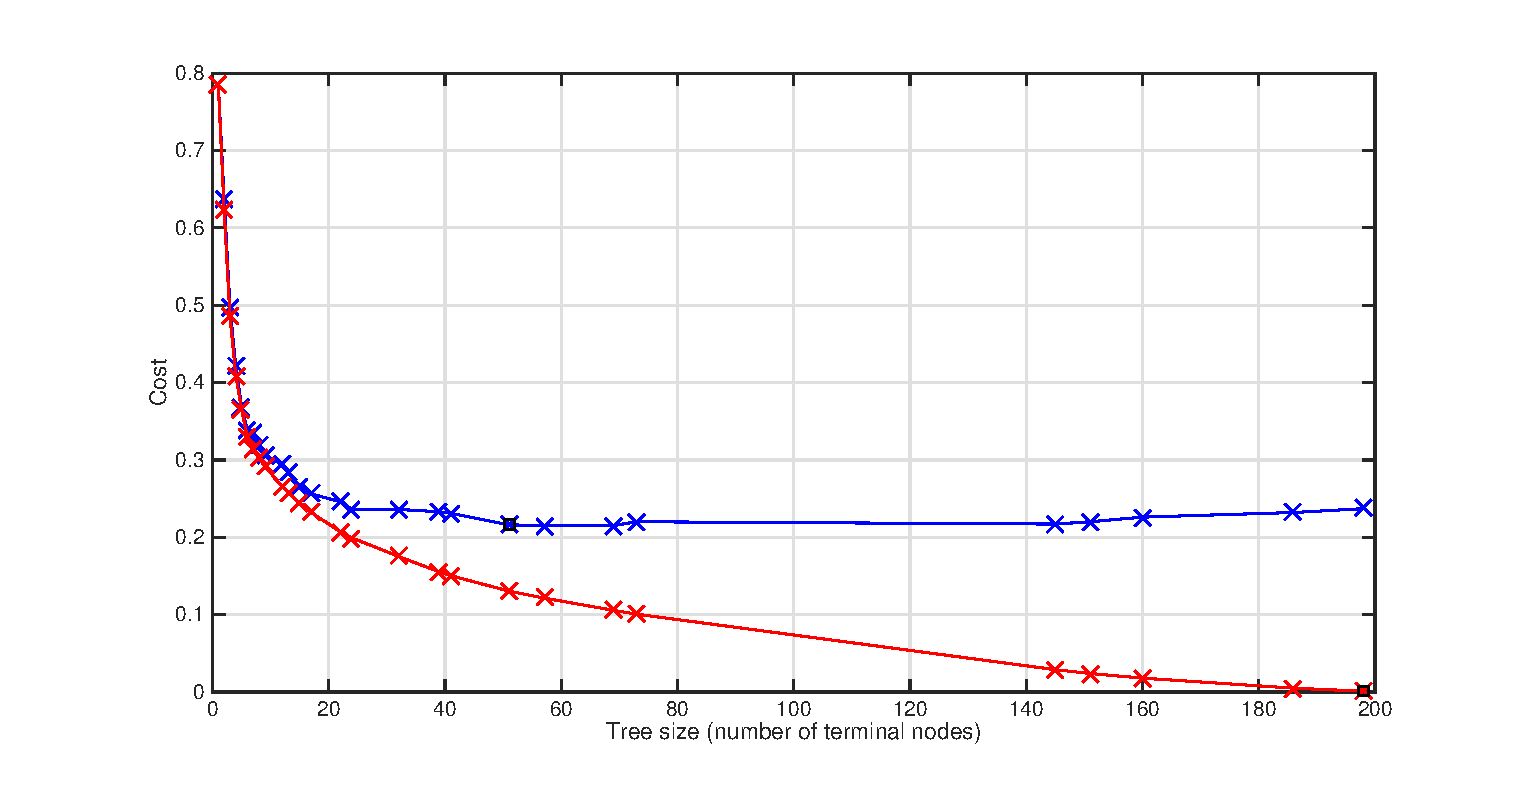
\includegraphics[scale=.4]{pruning_clean_data.eps}
}
\subcaptionbox{Pruning Example with noisy data}{
    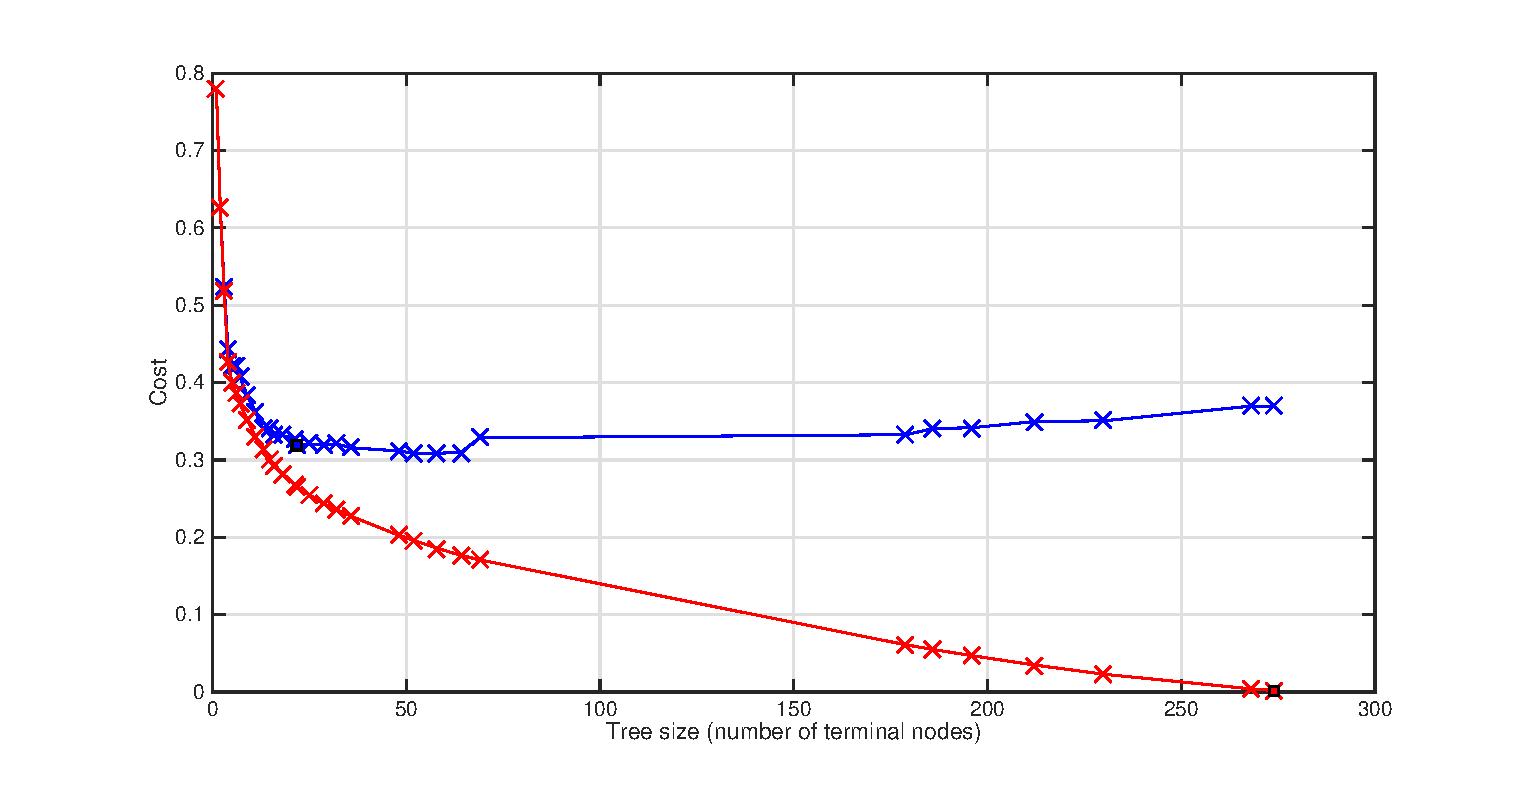
\includegraphics[scale=.4]{pruning_noisy_data.eps}
}
\end{figure}

These Figures show the error rate on validation and training set as the size (i. e. the number of leaves) of the trees increase.
For clean data the actual loss in accuracy is, as can be seen, negligible. With the optimal size, the error rate is 21\% instead of 24\% with no pruning.\\
For noisy data, this difference becomes much bigger. Pruning can increase performance in this case by approx. 10\% from 62\% to 68\%.

\section{Performance with Noisy Data}
The Performance with noisy data is much worse. Decision Trees can represent any kind of function, also the function generating noise. This is because while training the decision trees, we fit our tree to the training data, even if this data is noisy. Therefore noisy data generates noisy trees.
For Class 1 (precision is less than half in comparison to clean data) we especially have a problem of overfitting wich leads to much worse precision than with the clean data.

\section{Choosing the Best Algorithm}
We tested each of our algorithms using cross-validation. The Accuracy on the cross-validation test set is at this point a valid approximation of the accuracy on the unknown data set. On basis of these approximations, we choose the algorithm with the best accuracy.
After choosing an algorithm, we train it with the whole data set we got. Unfortunately, we don't have a test set to estimate the performance of this trained algorithm on unseen data.

\bibliographystyle{plainnat}
\bibliography{example}

\end{document}
